\documentclass[11pt]{beamer}
\usetheme{CambridgeUS}

%-----------------------------------------------------------------------
% Packages
\usepackage[utf8]{inputenc}
\usepackage{amsmath}
\usepackage{amsfonts}
\usepackage{amssymb}
\usepackage{graphicx}

%-----------------------------------------------------------------------
% Package customization
\definecolor{links}{HTML}{FC0D30}
\hypersetup{colorlinks,linkcolor=,urlcolor=links}

%-----------------------------------------------------------------------
% Commands
\renewcommand{\emph}[1]{\textbf{#1}}

%-----------------------------------------------------------------------
% Headings
\author{Marco Zanella}
\title{Object Oriented Programming}
\setbeamercovered{transparent} 
\setbeamertemplate{navigation symbols}{} 
\logo{
\includegraphics[width=.05\textwidth]{assets/logo-unipd}} 
\institute{University of Padova} 
\date{December, 9, 2024} 
\subject{Course Structure} 

%-----------------------------------------------------------------------
% Document
\begin{document}

\begin{frame}
\titlepage
\end{frame}

\begin{frame}{Overview}
 \begin{center}
  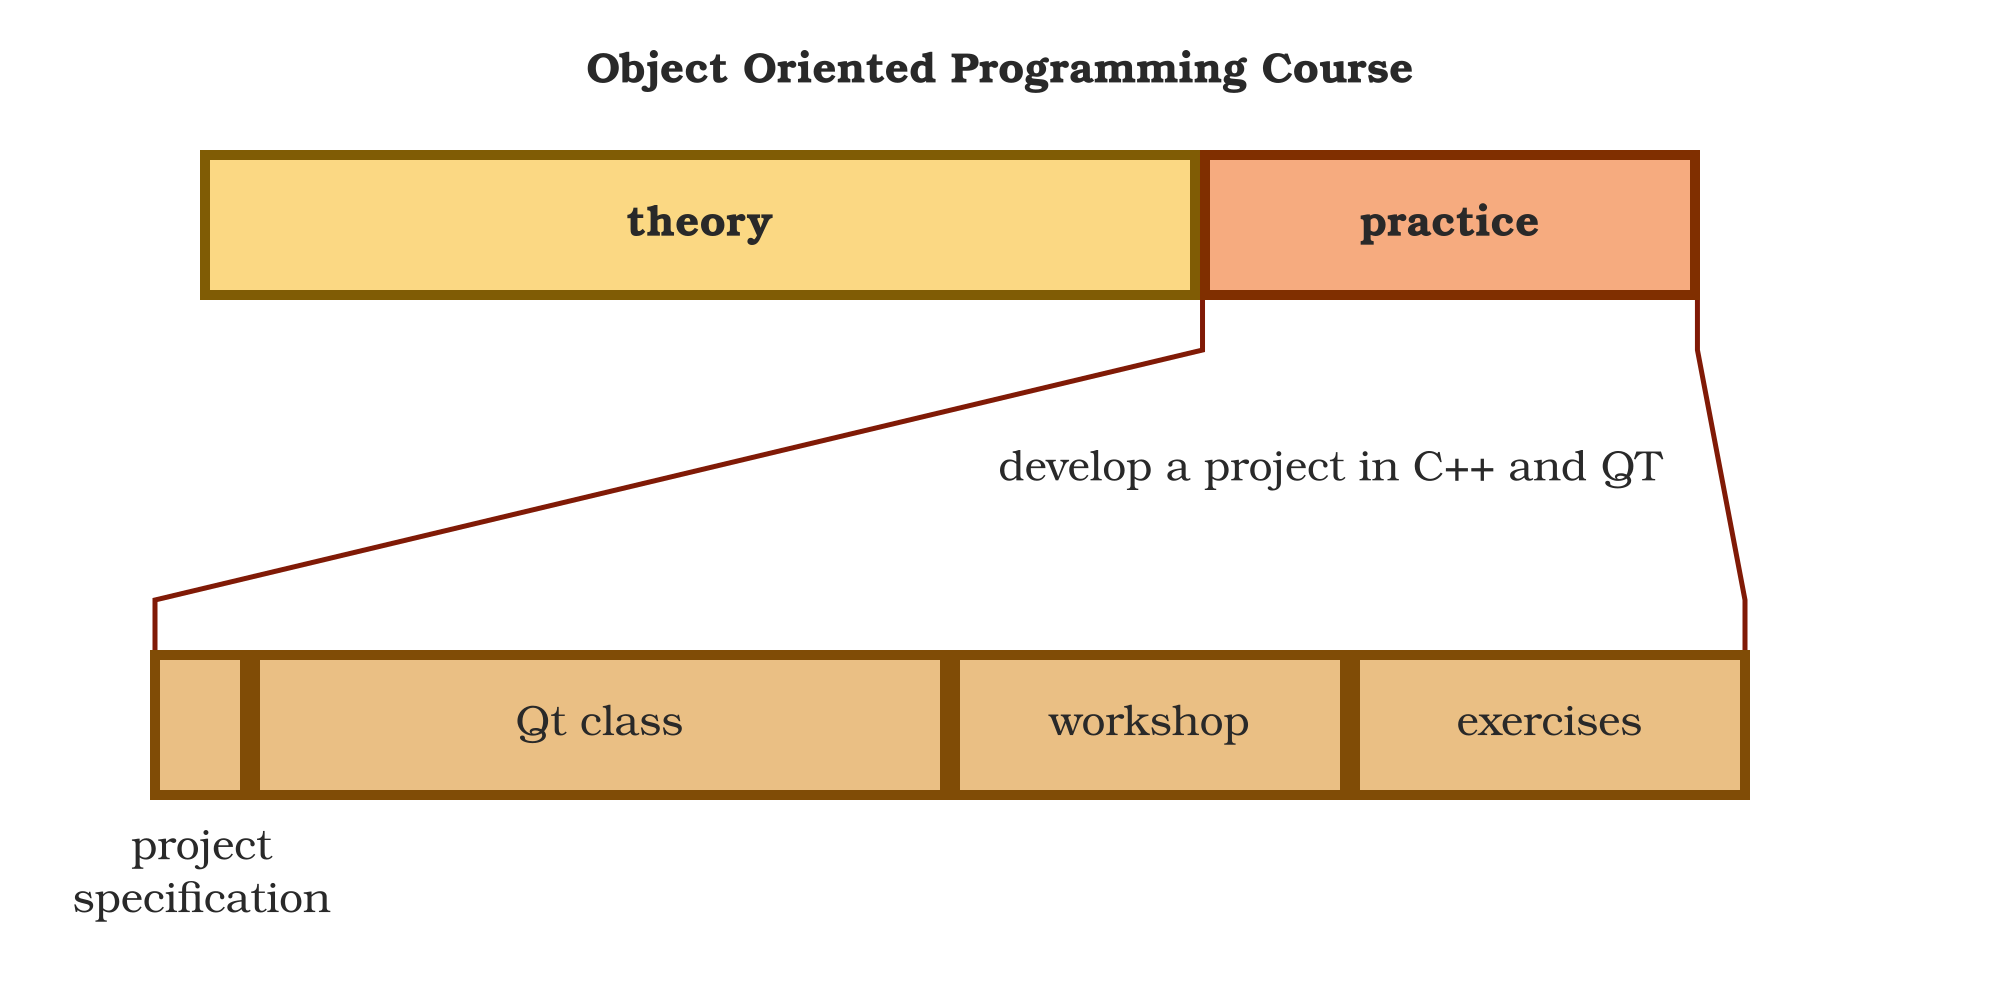
\includegraphics[width=1.0\textwidth]{assets/overview}
 \end{center}
\end{frame}

\begin{frame}{Schedule}
 \begin{center}
  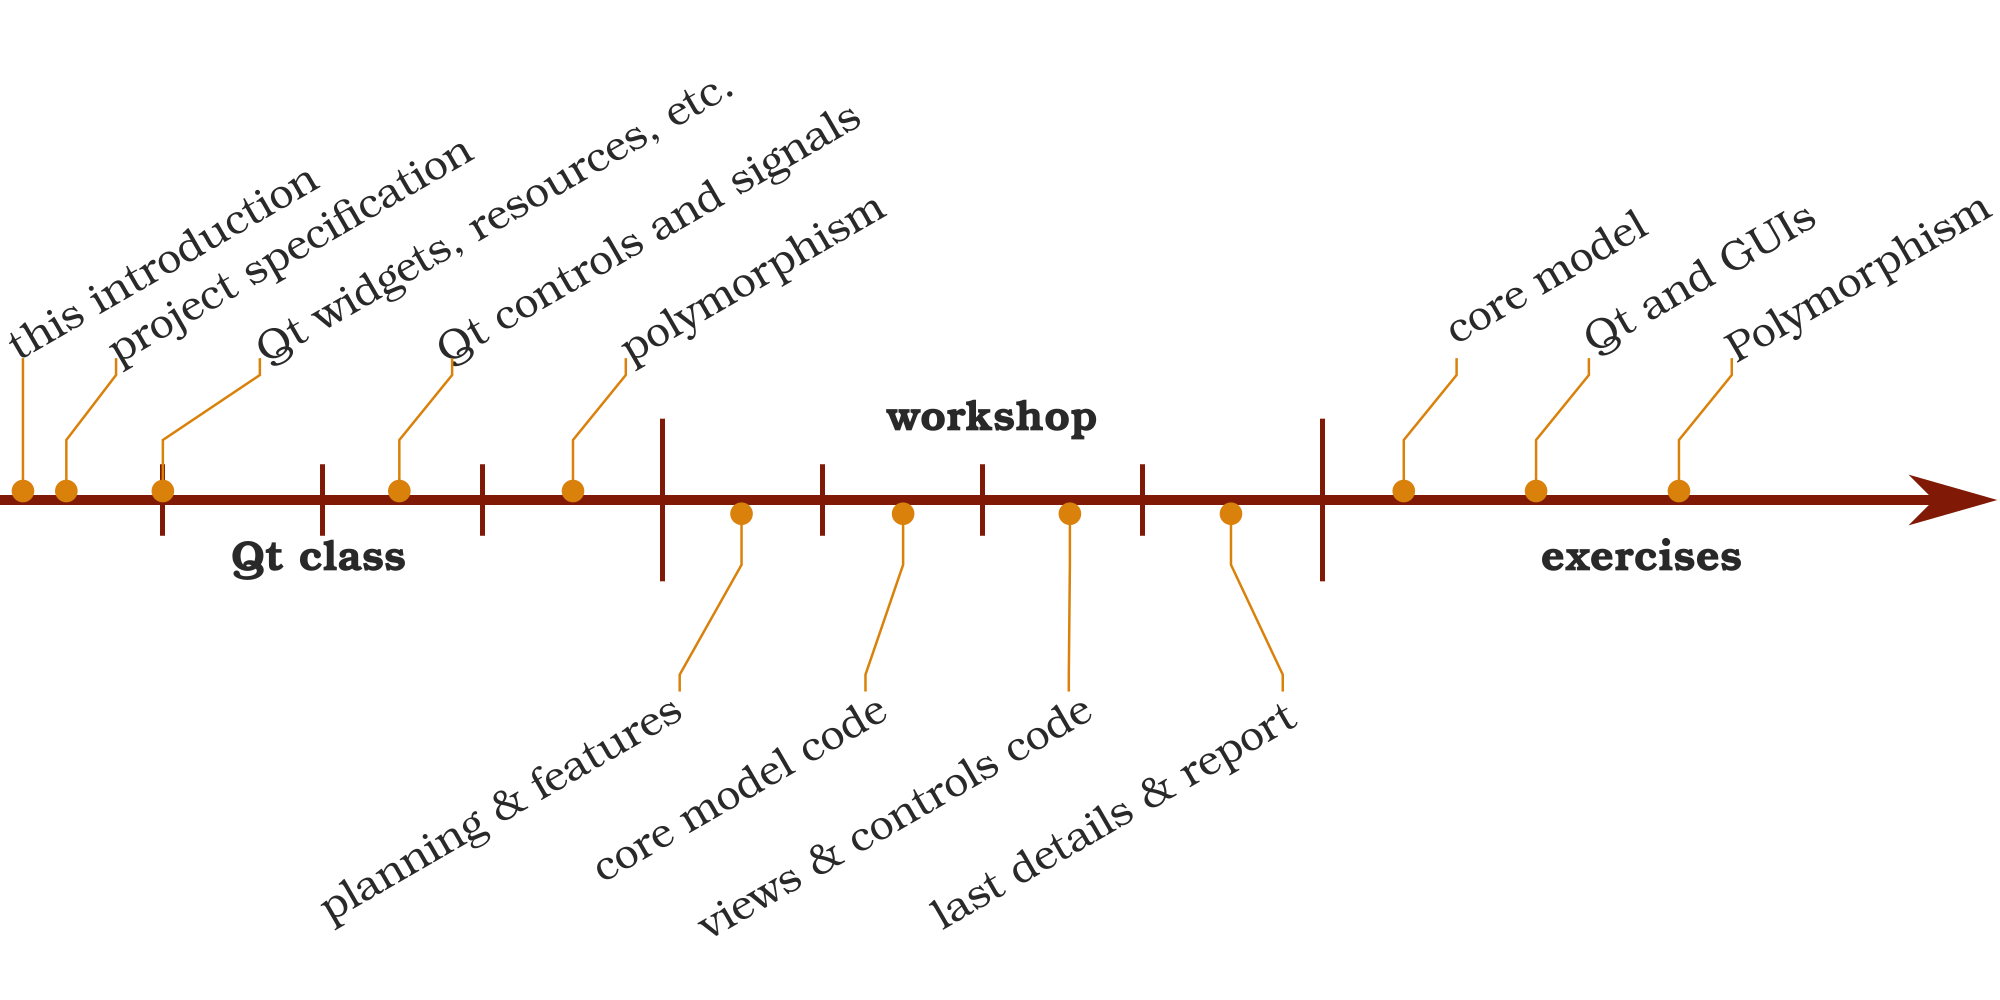
\includegraphics[width=1.0\textwidth]{assets/schedule}
 \end{center}
\end{frame}

\begin{frame}{Briefing}
 Keep in mind:
 \begin{itemize}
  \item theory exam \emph{unlocks practice}
  \item theory and practice \emph{evaluations are independent}
  \item project must satisfy \emph{constraints of this year}
  \item grade is valid for the \emph{whole academic year}
  \item you can work \emph{alone or in group} (max. 2 people)
 \end{itemize}
 You can find all the details about the project on Moodle \url{https://stem.elearning.unipd.it/course/view.php?id=6950}.
\end{frame}

\begin{frame}{Conclusion}
 For any issue, question or request:
 \begin{itemize}
  \item Moodle \url{https://stem.elearning.unipd.it/mod/forum/view.php?id=372887}
  \item email: \href{mailto:marco.zanella@unipd.it}{marco.zanella@unipd.it}
 \end{itemize}
 
 \begin{columns}
  \begin{column}{0.15\textwidth}
   
\includegraphics[width=0.99\textwidth]{assets/logo-github}
  \end{column}
  \begin{column}{0.85\textwidth}
   Source code, slides and other material also available at:
   \url{https://github.com/Unipd-Object-Oriented-Programming}
  \end{column}
 \end{columns}
\end{frame}

\end{document}
